\documentclass[11pt]{beamer}

\usepackage{epsfig}
\usepackage{amsfonts}
\usepackage{hyperref}
\usepackage[utf8x]{inputenc}
\usepackage{xkeyval}
%\usepackage{default}
\usepackage{estat-beamer}
\usepackage{amssymb,amsmath,url}


\title{A presentation on something incredibly interesting}
\subtitle{And Small Data}
\author{A.~N.~Onymous}
\institute{Methodology  and   Corporate  Architecture (ESTAT)}
\date{\today}

\begin{document}

% The [t] here aligns the title to the top of the slide, otherwise the
% author tends to end up in the picture on the lower right.
\frame[t]{\titlepage} % # 1

% ---------------------------------------------------------------------------------
% ---------------------------------------------------------------------------------

\frame { \frametitle{Frame I: A frame with a title longer than it has
    any reasonable right to expect to be}
  
  \begin{enumerate}
  \item Text 1
  \item Text 2
  \item Some longer text
  \item the longest text yet, even longer than the above, though why
    you would want to put in so much text is a whole other matter
  \end{enumerate}
}


% ---------------------------------------------------------------------------------
% ---------------------------------------------------------------------------------

\frame { \frametitle{A frame with images}
  
  \begin{columns}[totalwidth=\textwidth,T]
  \begin{minipage}{0.45\textwidth}
    \begin{column}[t]{\textwidth}
      \centering
      The background for the title slide:\\[0.5cm]
      
\includegraphics[width=\textwidth]{..//Eurostat_logo.jpg}
    \end{column}
\end{minipage}
  \begin{minipage}{0.45\textwidth}
    \begin{column}[t]{\textwidth}
      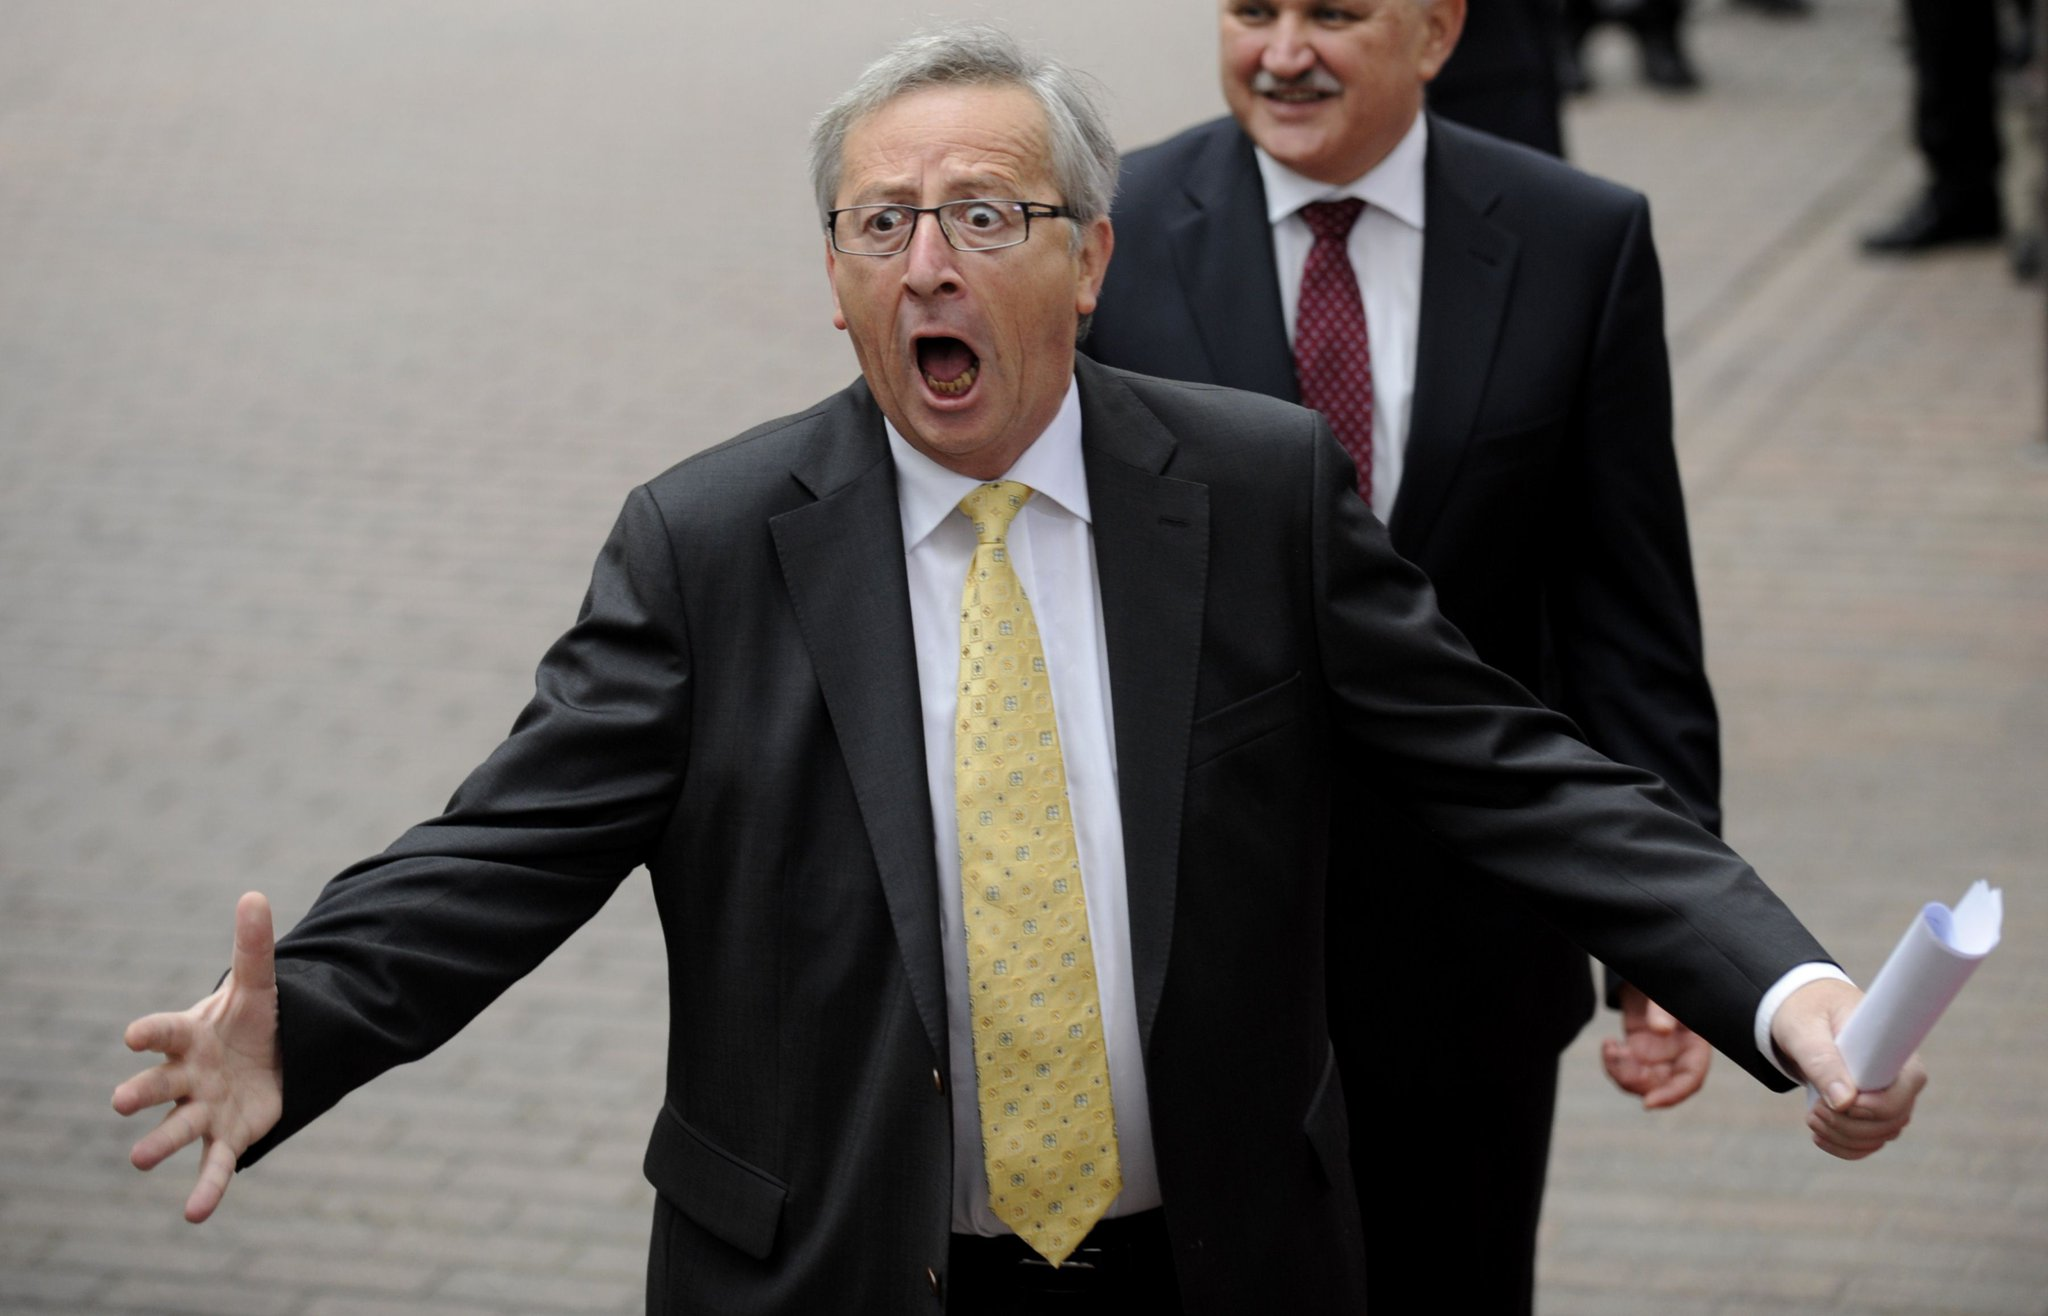
\includegraphics[width=\textwidth]{..//juncker.jpg}
      \centering
      fanstastic \\[0.5cm]
    \end{column}
\end{minipage}
  \end{columns}
  
}

% ---------------------------------------------------------------------------------
% ---------------------------------------------------------------------------------

\frame[c]{ \frametitle{A frame with tasty multifractal theory}
%% http://www.iacm.forth.gr/papers/grazzini_estimation_cp05.pdf

Under conditions of Fully Developed Turbulence, variables as
the velocity or the local dissipation of energy vary sharply from a location
to another and cannot be regarded as deterministic quantities but as random
ones. 

Let, for instance, $\epsilon_r(\vec{x})$ be the local dissipation of energy at the point
$\vec{x}$ over a neighbourhood of radius $r$:

    \[
\epsilon_r(\vec{x}) = \frac{1}{\mid B_r(\vec{x})\mid}
\int_{B_r(\vec{x})}
d\vec{x'} \sum_{i,j} [  \delta_i v_j(\vec{x'}) + \delta_j v_i(\vec{x'}) ]
 \]

with $v_i$  the components of the velocity vector and $B_r(\vec{x})$ the
ball of radius r centered around $\vec{x}$.
  
}
% ---------------------------------------------------------------------------------

\end{document}

